\section{RAVEN Theory by way of Examples: Forward Sampling Strategies}
In order to perform uncertainty quantification (UQ) and dynamic risk and
probabilistic assessment (D-PRA),
a sampling strategy needs to be employed. The sampling is aimed to
perturb the input space (domain of the uncertainties) in order to explore
the response of a complex system in relation to selected Figures of 
Merits (FOMs). 
\\The most widely used strategies to perform UQ and PRA are generally
collected into the category that, in RAVEN, is named \textit{\textbf{Forward}} samplers. The \textit{\textbf{Forward}} sampler category collects all the strategies that perform the sampling of the input space without exploiting, through dynamic learning approaches, the information made available from the outcomes of evaluation previously performed (adaptive sampling) and the common system evolution (patterns) that different sampled calculations can generate in the phase space (dynamic event tree). 
\\As mentioned in section \ref{par:ForwardSamplers}, RAVEN owns
different \textit{\textbf{Forward}} samplers, among which the most 
common are:
\begin{itemize}
  \item \textit{Monte-Carlo};
  \item \textit{Grid-based};
  \item \textit{Stratified} and its specialization, \textit{Latin Hyper Cube}.
\end{itemize}
In addition, RAVEN posses advanced \textit{\textbf{Forward}} sampling strategies that:
\begin{itemize}
  \item build a grid in the input space selecting evaluation points 
  based on characteristic quadratures as part of stochastic collocation 
  for generalized polynomial chaos method (\textit{Sparse 
  Grid Collocation} sampler);
  \item use high-density model reduction (HDMR) a.k.a. Sobol 
  decomposition to approximate a function as the sum of increasing-
  complexity interactions (\textit{Sobol} sampler).
\end{itemize} 
In the following subsections, the theory behind these sampling 
methodologies are going to be explained by way of applied RAVEN 
examples.

\subsection{Monte-Carlo}
\label{sub:MC}
The Monte-Carlo method is probably one of the most used methodologies in several disciplines. In this section, a brief theoretical 
background is reported. In addition,it is shown how to employ this methodology with RAVEN.
\subsubsection{Monte-Carlo theory introduction}
\label{subsub:MCtheory}
The Monte-Carlo method is aimed to approximate an expectation by the sample mean of a function of 
simulated random variables. It is based on the laws of large numbers in order to approximate expectations. 
In order words, it is aimed to approximate the average response of multiple FOMs 
relying on multiple random sampling of the input space. 
\\Let's consider a random variable (eventually multidimensional) $\bar{x}$ having probability mass function or probability density function $pdf_{X}(x)$,
which is greater than zero on a set of values $\chi$. Then the expected value of a function $f$ of $X$ is as follows:
\begin{equation}
\begin{matrix}
\mathbb{E}(f(X)) =\sum_{x \in \chi} f(x)pdf_{X}(x) & if X \, discrete \\ 
\\ 
\mathbb{E}(f(X)) =\int_{x \in \chi} f(x)pdf_{X}(x) & \, if X \, \, continuous
\end{matrix}
\end{equation}
Let's now consider to take an $n$-sample of $X$, $(x_{1},...,x_{n})$, and compute the mean of $f(x)$ over the samples. This computation represents the Monte-Carlo estimate:
\begin{equation}
  \mathbb{E}(f(X)) \approx   \widetilde{f}_{n}(x) = \frac{1}{n} \sum_{i=1}^{n} f(x_{i})  
\end{equation}
If $\mathbb{E}(f(X))$ exists, then the law of large numbers determines that for any arbitrarily small $\varepsilon$:
\begin{equation}
  \lim_{n\rightarrow \, \infty} P( \left | \widetilde{f}_{n}(X) - \mathbb{E}(f(X))  \right |\geq \varepsilon) = 0
\end{equation}
The above equation suggests that as $n$ gets larger, then the probability that $\widetilde{f}_{n}(X)$ deviates 
from the $\mathbb{E}(f(X))$ becomes smaller. In other words, more samples are spooned, more closer the Monte-Carlo estimate of $X$ gets to the real value.
\\In addition $\widetilde{f}_{n}(X)$ represent an unbiased estimate for $\mathbb{E}(f(X))$:
\begin{equation}
\mathbb{E}(\widetilde{f}_{n}(X)) = \mathbb{E} \left ( \frac{1}{n} \sum_{i=1}^{n} f(x_{i})   \right ) = 
\frac{1}{n} \sum_{i=1}^{n} \mathbb{E}(f(x_{i})) =   \mathbb{E}(f(X)) 
\end{equation}
After this brief introduction, it is important to understand how the Monte-Carlo method can be employed 
for the analysis of Dynamic Stochastic system.
\\Referencing to the nomenclature defined in section~\ref{sub:mathBackground}, given:
\begin{equation}
\frac{\partial  \overline{\theta}^{c}\left ( t \right )}{\partial t}=f\left ( \overline{\theta}^{c},\overline{\theta}^{d}_{i}, \overline{\alpha}_{staz} ,\overline{\alpha}_{brow}, t \right )
\end{equation}
let's define a function $g_{i}$ that represents the solution of the previous equation (the trajectory in the $ \overline{\theta}^{c}$ space for a fixed $ \overline{\theta}^{d}_{i}$ and initial condition $\overline{\theta}^{c}_{0}$) :
\begin{equation}
  \overline{\theta}^{c}(t) = g_{i}(t,\overline{\theta}^{c}_{0})
\end{equation}
The Monte-Carlo analysis is performed as following:
\begin{enumerate}
  \item Sample:
  \begin{itemize}
    \item $\overline{\alpha}_{staz} $,$\overline{\alpha}_{DS}$, $\overline{t}$ depending on which 
    approximations are valid (see~\ref{sub:mathBackground});
    \item The initial conditions $\overline{\theta}^{c}_{0}$,$\overline{\theta}^{d}_{0}$;
    \item Transition conditions from $W(\overline{\theta}^{d}|\overline{\theta}^{d}_{i},\overline{\theta}^{c},t)$
  \end{itemize}
  \item Run the system simulator using the previously sampled values and affected by the intrinsic stochasticity 
  represented by $\overline{\alpha}_{brow}$;
  \item Pause the simulation when a transition condition is reached and move from the current $\overline{\theta}^{d}_{0}$ to the new $\overline{\theta}^{d}$ (e.g. $\overline{\theta}^{d}_{1}$);
  \item Run the simulation as performed in step 3, starting from the new coordinate and pause the simulation when a new transition is reached;
  \item Repeat steps 3 and 4 until a stopping condition is reached;
  \item Repeat 1 through 4 for a large number of runs $n$.
\end{enumerate}



\subsubsection{Monte-Carlo sampling through RAVEN}
\label{subsub:MCexample}
The goals of this section are about learning how to:
 \begin{enumerate}
   \item Set up a simple Monte-Carlo sampling for perturbing the input space of a driven code;
   \item Load the outputs of the code into the RAVEN DataObjects system;
   \item Print out what contained in the DataObjects;
   \item Generate basic plots of the code results.
\end{enumerate}  
In order to accomplish these tasks, the following RAVEN \textbf{Entities} (XML blocks in the input files) need to be defined:
 \begin{enumerate}
   \item \textbf{\textit{RunInfo}}:
\begin{lstlisting}[style=XML,morekeywords={arg,extension,pauseAtEnd,overwrite}]
    <RunInfo>
      <Sequence>Single, write-History</Sequence>
      <WorkingDir>sectionVI.I</WorkingDir>
      <batchSize>1</batchSize>
    </RunInfo>   
\end{lstlisting}   
   As reported in section~\ref{sub:EntitiesAndFlow}, the \textit{RunInfo} \textbf{Entity} is intended to set up the analysis 
   that the user wants to perform. In this specific case, two steps (\xmlNode{Sequence}) are going to be sequentially run 
   using a single processor (\xmlNode{batchSize}).
   
   \item \textbf{\textit{Files}}:
\begin{lstlisting}[style=XML,morekeywords={arg,extension,pauseAtEnd,overwrite}]
  <Files>
    <Input name="referenceInput.xml" type="input">referenceInput.xml</Input>
  </Files>
\end{lstlisting}
   Since the driven code uses a single input file, in this section the original input is placed. As detailed in the user manual
   the attribute  \xmlAttr{name} represents the alias that is going to be used in all the other input blocks in order to 
   refer to this file.
   \item \textbf{\textit{Models}}:
\begin{lstlisting}[style=XML,morekeywords={arg,extension,pauseAtEnd,overwrite}]
   <Models>
      <Code name="testModel" subType="GenericCode">
        <executable>
          ../physicalCode/analyticalbateman/AnalyticalDplMain.py
        </executable>
        <clargs arg="python" type="prepend"/>
        <clargs arg="" extension=".xml" type="input"/>
        <clargs arg="" extension=".csv" type="output"/>
        <prepend>python</prepend>
      </Code>
    <Models>
\end{lstlisting}
  As already mentioned, since the driven code already dumps its outputs in CSV format, there is no need to create
  an ad-hoc code interface and the GenericCode interface can be directly used. Since the \textbf{AnalyticBateman} code
  is written in python, it is necessary to specify that the code needs to be run pre-pending the expression ``python''. 
   \item \textbf{\textit{DataObjects}}:
\begin{lstlisting}[style=XML,morekeywords={arg,extension,pauseAtEnd,overwrite}]
  <DataObjects>
    <PointSet name="pointValues">
      <Input>InputPlaceHolder</Input>
      <Output>A,B,C,D</Output>
    </PointSet>
    <HistorySet name="history">
        <Input>InputPlaceHolder</Input>
        <Output>A,B,C,D,time</Output>
    </HistorySet>
  </DataObjects>
\end{lstlisting}
  Int this block, two \textit{DataObjects} are defined: 1) PointSet named ``pointValues'', 2) HistorySet named ``history''.
  As it can be noticed, a special keyword is inputted in the \xmlNode{Input} node. This keyword is used when a \textit{DataObjects}  \textbf{Entity} needs to be constructed without any linking with respect to the input space. Indeed, in 
  this case, the model input space is not perturbed though a sampling strategies; the code is executed through the original
   input file   (``referenceInput.xml''). In the \xmlNode{Output} node all the requested variables are inputted.
   \item \textbf{\textit{OutStreamManager}}:   
\begin{lstlisting}[style=XML,morekeywords={arg,extension,pauseAtEnd,overwrite}]
  <OutStreamManager>
    <Print name="pointValues">
      <type>csv</type>
      <source>pointValues</source>
    </Print>
    <Print name="history">
        <type>csv</type>
        <source>history</source>
    </Print>
    <Plot dim="2" name="historyPlot" overwrite="false" verbosity="debug">
        <plotSettings>
            <plot>
                <type>line</type>
                <x>history|Output|time</x>
                <y>history|Output|A</y>
                <color>blue</color>
            </plot>
            <plot>
                <type>line</type>
                <x>history|Output|time</x>
                <y>history|Output|B</y>
                <color>red</color>
            </plot>
            <plot>
                <type>line</type>
                <x>history|Output|time</x>
                <y>history|Output|C</y>
                <color>yellow</color>
            </plot>
            <plot>
                <type>line</type>
                <x>history|Output|time</x>
                <y>history|Output|D</y>
                <color>black</color>
            </plot>
            <xlabel>time (s)</xlabel>
            <ylabel>evolution (kg)</ylabel>
        </plotSettings>
        <actions>
            <how>png,screen</how>
            <title>
                <text> </text>
            </title>
        </actions>
    </Plot>
  </OutStreamManager>
\end{lstlisting}
  In this block, both the Out-Stream types are constructed: 
  \begin{itemize}
    \item \textit{Print}: 
     \begin{itemize}
       \item named ``pointValues'' connected with the \textit{DataObjects} \textbf{Entity} ``pointValues'' 
                (\xmlNode{source})
       \item named ``history'' connected with the \textit{DataObjects} \textbf{Entity} ``history'' (\xmlNode{source})          
     \end{itemize}         
      When this objects get used, all the information contained in the linked  \textit{DataObjects} are going 
    to be dumped in CSV files (\xmlNode{type}).
    \item \textit{Plot}: a single \xmlNode{Plot} \textbf{Entity} is defined, containing the line plots of the 4 output variables 
    ($A,B,C,D$) in the same figure. As it can be seen, this object is going to generate a PNG file and an interactive Plot on 
    the screen.
  \end{itemize}   
   \item \textbf{\textit{Steps}}:   
\begin{lstlisting}[style=XML,morekeywords={arg,extension,pauseAtEnd,overwrite}]
  <Steps>
    <SingleRun name="Single">
      <Input   class="Files"                        type="input">referenceInput.xml</Input>
      <Model  class="Models"                    type="Code">testModel</Model>
      <Output class="DataObjects"            type="PointSet">pointValues</Output>
      <Output class="DataObjects"            type="HistorySet">history</Output>
      <Output class="OutStreamManager" type="Print">pointValues</Output>
    </SingleRun>
    <IOStep name="writeHistory" pauseAtEnd="True">
        <Input    class="DataObjects"            type="HistorySet">history</Input>
        <Output class="OutStreamManager" type="Print">history</Output>
        <Output class="OutStreamManager" type="Plot">historyPlot</Output>
    </IOStep>
  </Steps>
\end{lstlisting}
 %%%%%%%%%%%%%%%%%%%%%%%%%%%%%%%%%%%%%%%%%%%%%%%%%%%%%%%%%%
 %figure history
 \begin{figure}[h!]
  \centering
  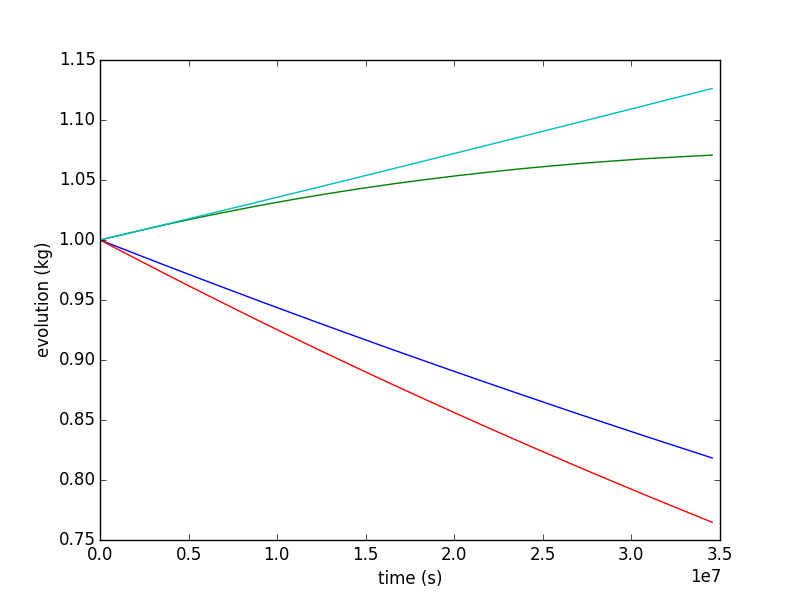
\includegraphics[scale=0.7]{pics/1-historyPlot_line-line-line-line.png}
  \caption{Plot of the history for variables $A,B,C,D$.}
  \label{fig:historyPlotLine}
 \end{figure}
 %%%%%%%%%%%%%%%%%%%%%%%%%%%%%%%%%%%%%%%%%%%%%%%%%%%%%%%%%%
   Finally, all the previously defined \textbf{Entities} can be combined in the \xmlNode{Steps} block. As inferable, 
   two \xmlNode{Steps} have been inputted:
   \begin{itemize}
     \item \xmlNode{SingleRun} named ``Single'', used to run the single instance of the driven code and collect 
     the outputs in the two \textit{DataObjects}. In addition, it can be seen that an additional object has been  
     placed among the \xmlNode{Output}(s).Indeed, an  \textit{OutStreamManager} can be an \xmlNode{Output} in 
     any Step type (as long as the linked \textit{DataObjects} plays a whatever role in the Step);
     \item  \xmlNode{IOStep} named ``writeHistory'', used to 1) dump the ``history'' \textit{DataObjects} 
     \textbf{Entity} in a CSV file and 2) plot the data in the PNG file and on the screen.
   \end{itemize}
\end{enumerate} 
 Tables~\ref{pointValuesVI.I} and \ref{historyVI.I} show the results dumped by the OutStreams \textit{Print}.
 As previously mentioned, Figure~\ref{fig:historyPlotLine} reports the 4 plots (4 variables) drawn in the same picture. 
 % table history set
\begin{table}[h!]
\centering
\caption{``history'' HistorySet CSV output file.}
\label{historyVI.I}
\begin{tabular}{|c|c|c|c|c|}
\hline
\textbf{A}                        & \textbf{C}                       & \textbf{B}                       & \textbf{D}                       & \textbf{time}                 \\ \hline
1                                 & 1                                & 1                                & 1                                & 0                             \\ \hline
0.983434738                       & 0.977851848                      & 1.010115067                      & 1.010131723                      & 2880000                       \\ \hline
0.967143884                       & 0.956202457                      & 1.019362317                      & 1.020361004                      & 5760000                       \\ \hline
0.951122893                       & 0.935040451                      & 1.027774063                      & 1.03067926                       & 8640000                       \\ \hline
0.941637969                       & 0.922572556                      & 1.032433141                      & 1.036909471                      & 10368000                      \\ \hline
0.932247632                       & 0.910273757                      & 1.036809334                      & 1.043167001                      & 12096000                      \\ \hline
0.922950939                       & 0.89814173                       & 1.040909121                      & 1.049450159                      & 13824000                      \\ \hline
0.913746955                       & 0.886174184                      & 1.044738857                      & 1.055757293                      & 15552000                      \\ \hline
0.904634757                       & 0.874368858                      & 1.048304784                      & 1.062086789                      & 17280000                      \\ \hline
0.886682065                       & 0.851235987                      & 1.054669586                      & 1.074806592                      & 20736000                      \\ \hline
0.869085647                       & 0.828725659                      & 1.060051155                      & 1.087597391                      & 24192000                      \\ \hline
\multicolumn{1}{|l|}{0.851838435} & \multicolumn{1}{l|}{0.806820897} & \multicolumn{1}{l|}{1.064495355} & \multicolumn{1}{l|}{1.100447571} & \multicolumn{1}{l|}{27648000} \\ \hline
\multicolumn{1}{|l|}{0.834933498} & \multicolumn{1}{l|}{0.785505192} & \multicolumn{1}{l|}{1.068046343} & \multicolumn{1}{l|}{1.113346061} & \multicolumn{1}{l|}{31104000} \\ \hline
\multicolumn{1}{|l|}{0.818364044} & \multicolumn{1}{l|}{0.764762489} & \multicolumn{1}{l|}{1.070746628} & \multicolumn{1}{l|}{1.126282318} & \multicolumn{1}{l|}{34560000} \\ \hline
\end{tabular}
\end{table} 
% table point set
\begin{table}[h!]
\centering
\caption{``pointValues'' PointSet CSV output file.}
\label{pointValuesVI.I}
\begin{tabular}{|c|c|c|c|c|}
\hline
\textbf{InputPlaceHolder} & \textbf{A}    & \textbf{C}     & \textbf{B}    & \textbf{D}    \\ \hline
0.0                       & 0.81836404385 & 0.764762489077 & 1.07074662835 & 1.12628231792 \\ \hline
\end{tabular}
\end{table}


\subsection{Single Run using the OutStream system to sub-plot and selectively print.}
In this section, the user can learn how to use RAVEN to create sub-plots (multiple plots in the same figure) and 
how to select only some variable from the \textit{DataObjects} in the \textit{Print} OutStream.
 \\ The goals of this section are about learning how to:
 \begin{enumerate}
   \item Print out what contained in the DataObjects, selecting only few variables;
   \item Generate sub-plots (multiple plots in the same figure) of the code results.
\end{enumerate}  

In order to accomplish these tasks, the \textit{OutStreamManager} \textbf{Entity} in the input defined in the previous section (~\ref{sub:SingleRunBasicPlots}) needs to be modified as follows:
\begin{enumerate}
   \item \textbf{\textit{Print}}:
   \begin{lstlisting}[style=XML,morekeywords={arg,extension,pauseAtEnd,overwrite}]
    <Print name="pointValues">
      <type>csv</type>
      <source>pointValues</source>
      <what>Output</what>
    </Print>
    <Print name="history">
        <type>csv</type>
        <source>history</source>
        <what>Output|A,Output|D</what>
    </Print>
   \end{lstlisting}   
   With respect to the \textit{Print} nodes defined in the previous section (~\ref{sub:SingleRunBasicPlots}), it can
   be noticed that an additional node has been added: \xmlNode{what}. The \textit{Print} \textbf{Entity}  
   ``pointValues'' is going to extract and dump only the variables that are part of the Output space 
   ($A,B,C,D$ and not $InputPlaceHolder$).  The \textit{Print} \textbf{Entity} ``history'' is instead going to print 
   the Output space variables $A$ and $D$. 

   \item \textbf{\textit{Plot}}:
   \begin{lstlisting}[style=XML,morekeywords={arg,extension,pauseAtEnd,overwrite}]
    <Plot dim="2" name="historyPlot" overwrite="false" verbosity="debug">
        <plotSettings>
            <gridSpace>2 2</gridSpace>
            <plot>
                <type>line</type>
                <x>history|Output|time</x>
                <y>history|Output|A</y>
                <color>blue</color>
                <gridLocation>
                  <x>0</x>
                  <y>0</y>
                </gridLocation>
            </plot>
            <plot>
                <type>line</type>
                <x>history|Output|time</x>
                <y>history|Output|B</y>
                <color>red</color>
                <gridLocation>
                    <x>1</x>
                    <y>0</y>
                </gridLocation>
            </plot>
            <plot>
                <type>line</type>
                <x>history|Output|time</x>
                <y>history|Output|C</y>
                <color>yellow</color>
                <gridLocation>
                    <x>0</x>
                    <y>1</y>
                </gridLocation>
            </plot>
            <plot>
                <type>line</type>
                <x>history|Output|time</x>
                <y>history|Output|D</y>
                <color>black</color>
                <gridLocation>
                    <x>1</x>
                    <y>1</y>
                </gridLocation>
            </plot>
            <xlabel>time (s)</xlabel>
            <ylabel>evolution (kg)</ylabel>
        </plotSettings>
        <actions>
            <how>png,screen</how>
            <title>
                <text> </text>
            </title>
        </actions>
    </Plot>
\end{lstlisting}   
 As it can be noticed, the  \textit{Plot} \textbf{Entity} does not differ much with respect to the one in 
 section~\ref{sub:SingleRunBasicPlots}: 1) the additional sub-node \xmlNode{gridSpace}  has been added. 
 This node is needed to define how the figure needs to be partitioned (discretization of the grid). In this case
 a 2 by 2 grid is requested. 2) in each \xmlNode{plot} the node \xmlNode{gridLocation} needs to be placed in 
 order to specify in which position the relative plot needs to be placed. For example, in the following grid 
 location, the relative plot is going to be placed at the bottom-right corner.
  \begin{lstlisting}[style=XML,morekeywords={arg,extension,pauseAtEnd,overwrite}]
   <gridLocation>
      <x>1</x>
      <y>1</y>
   </gridLocation>
   \end{lstlisting}   
 \end{enumerate}
The CSV tables generated by the \textit{Print} \textbf{Entities} are not reported, since the only differences with respect to the  tables~\ref{pointValuesVI.I} and \ref{historyVI.I} are related to the number of columns (variables)
dumped out. 
\\Figure~\ref{fig:historySubPlotLine} reports the 4 plots (4 variables) drawn in the same picture. 
 %figure history sublots
 \begin{figure}[h!]
  \centering
  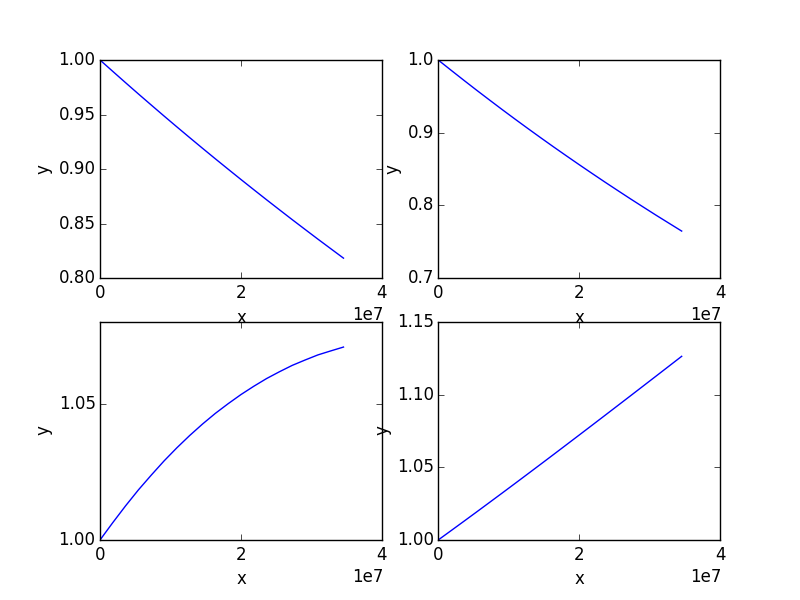
\includegraphics[scale=0.7]{pics/1-historyPlot_line-line-line-line-subPlots.png}
  \caption{Sub-plot of the history for variables $A,B,C,D$.}
  \label{fig:historySubPlotLine}
 \end{figure}

\subsection{Grid}
\label{sub:Grid}
The Grid sampling method (also known as Full Factorial Design of 
Experiment) represents one of the simplest methodologies that can be 
employed in order to explore the interaction of multiple random 
variables with respect to selected FOMs.
In this section, a brief theoretical 
background is reported. In addition,it is shown how to employ this methodology with RAVEN.
\subsubsection{Grid theory introduction}
\label{subsub:Gridtheory}
As already mentioned, the Grid-based sampling strategy is aimed to
explore the interaction of multiple random variables (i.e. uncertainties) 
with respect to selected FOMs.